\chapter{Estado del arte}

Antes de seguir, me veo en la obligación de hablar un poco sobre conceptos generales en el mundo del deporte. Un ejercicio, es la repetición de un movimiento varias veces para estimular uno o varios músculos. Los entrenamientos, entendámolos como la colección de distintos ejercicios destinados a entrenar una parte o varias del cuerpo, a los entrenamientos también se les llama rutinas. Una serie, es cuando dentro de un ejercicio, repetimos ese movimiento un número determinado de veces y se realiza un descanso, sin cambiar de ejercicio.Una repetición, es la realización del movimiento de ese ejercicio en una serie, es decir, si estoy haciendo flexiones, hago 12, descanso, hago 10, descanso, hago 9 y ya no hago más flexiones, dentro de mi entrenamiento se vería así:

\underline {Rutina de entrenamiento 1:}
\begin{itemize}
	\item Ejercicio 1
	\begin{itemize}
		\item Serie 1: X repeticiones
		\item Serie 2: X repeticiones
	\end{itemize}
	\item Flexiones
	\begin{itemize}
		\item Serie 1: 12 repeticiones
		\item Serie 2: 10 repeticiones 
		\item Serie 3: 9 repeticiones
	\end{itemize}
	\item Ejercicio 3
	\begin{itemize}
		\item Serie 1: X repeticiones
		\item Serie 2: X repeticiones
	\end{itemize}
\end{itemize}

\section{Aplicaciones similares}

Algunas de las aplicaciones que existen, para mediciones de constantes relacionadas durante el entrenamiento físico, suelen ser de pago. Ejemplos de precios mensuales:

\begin{itemize}
	\item \textbf{Fitbit Premium: €9.99}, esta app ofrece una interfaz para medir constantes usando un smartwatch con sensor cardíaco (ritmo cardíaco, calorías quemadas, pasos, ect). En lo que respecta que es el entrenamiento, solo ofrece una serie de entrenamiento prefijados, además no permite guardar resultados.
\begin{figure}[H]
   \centering
    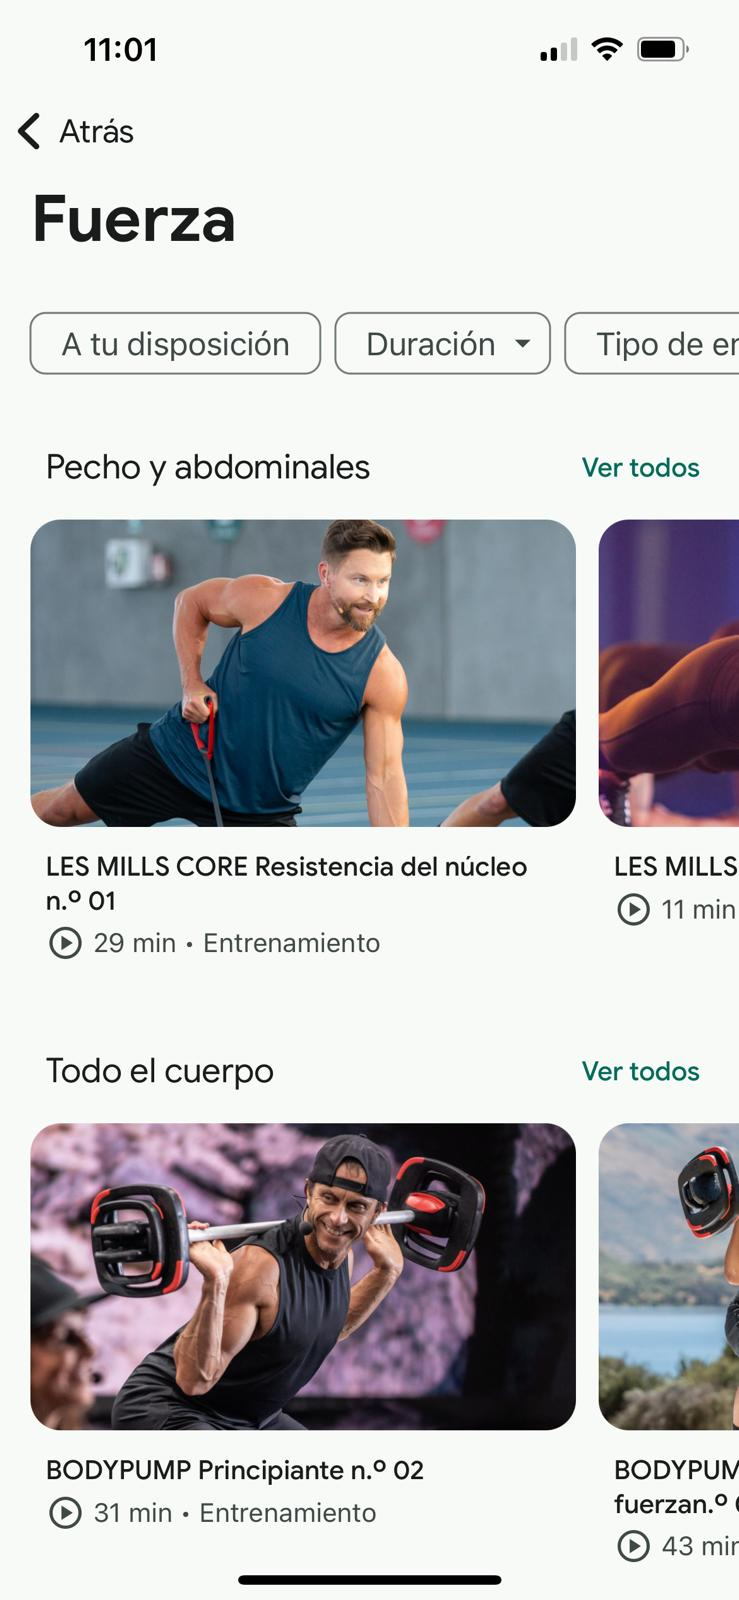
\includegraphics[width=0.5\textwidth]{fotos/fitbit.jpeg}
    \caption{Fitbit}
    \label{fig:Fitbit}
\end{figure} 
	\item \textbf{Apple Fitness+: €9.99}, en su verión gratuita nos permite guardar todas las variables permitidas con un smartwatch, las registra y va aconsejando, si detecta que tienes estres salta un aviso, poco movimiento, pulsaciones anormales, etc. En la versión de pago añade los entrenamientos, pero vuelve a la misma problemática, son entrenamientos prefijados y no permite guardar tu rendimiento.
\begin{figure}[H]
   \centering
    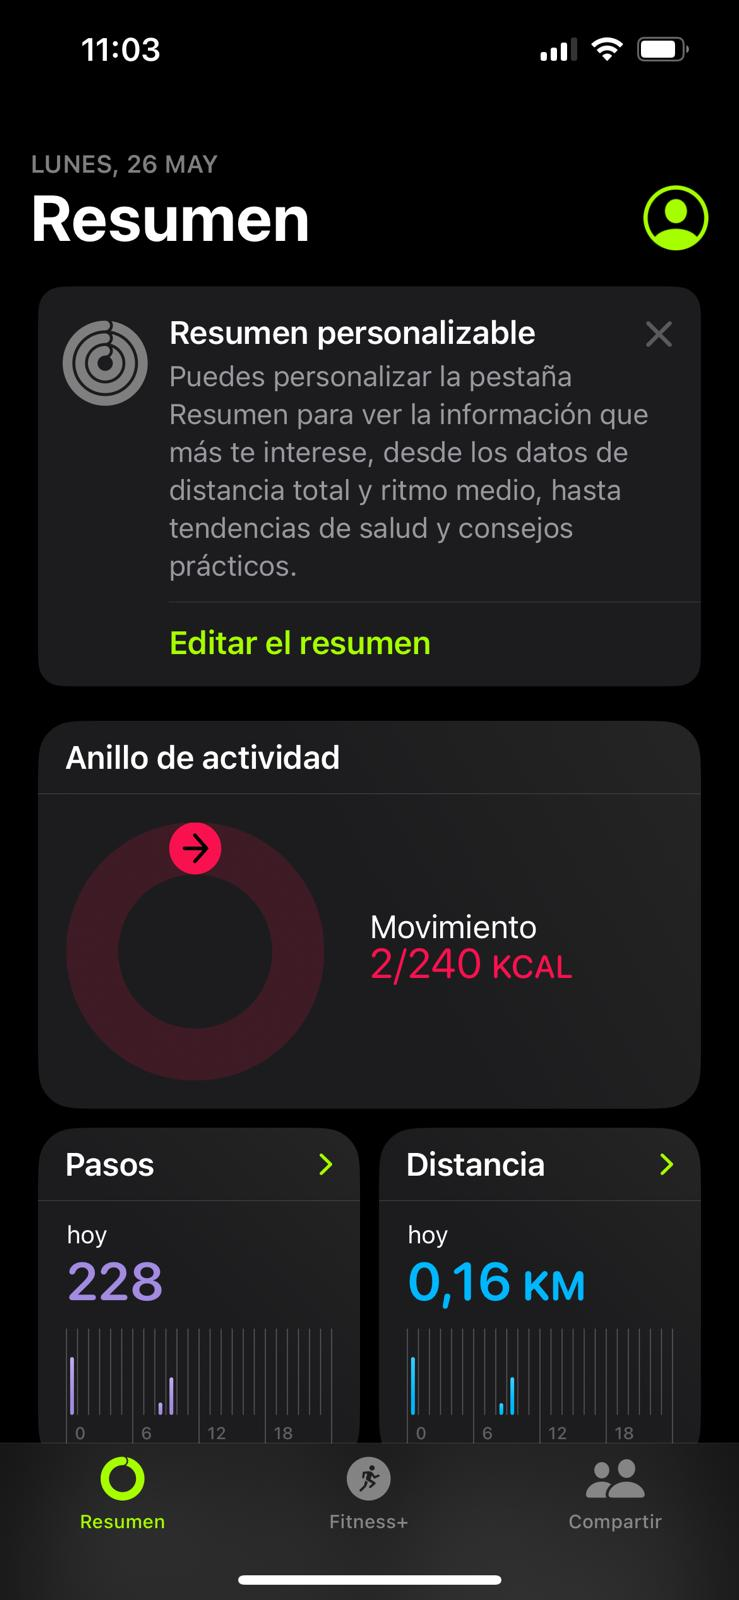
\includegraphics[width=0.5\textwidth]{fotos/fitness.jpeg}
    \caption{Apple fitness}
    \label{fig:Apple fitness}
\end{figure} 
	\item \textbf{Strava Premium: €5.99}, es una app más enfocada a running, pero permite medir variables relacionadas con este tipo de entrenamientos, kilómetros recorridos, rítmo, ruta recorrida, tiempo, etc. Es muy completa solo para ese tipo de entrenamientos.
\begin{figure}[H]
   \centering
    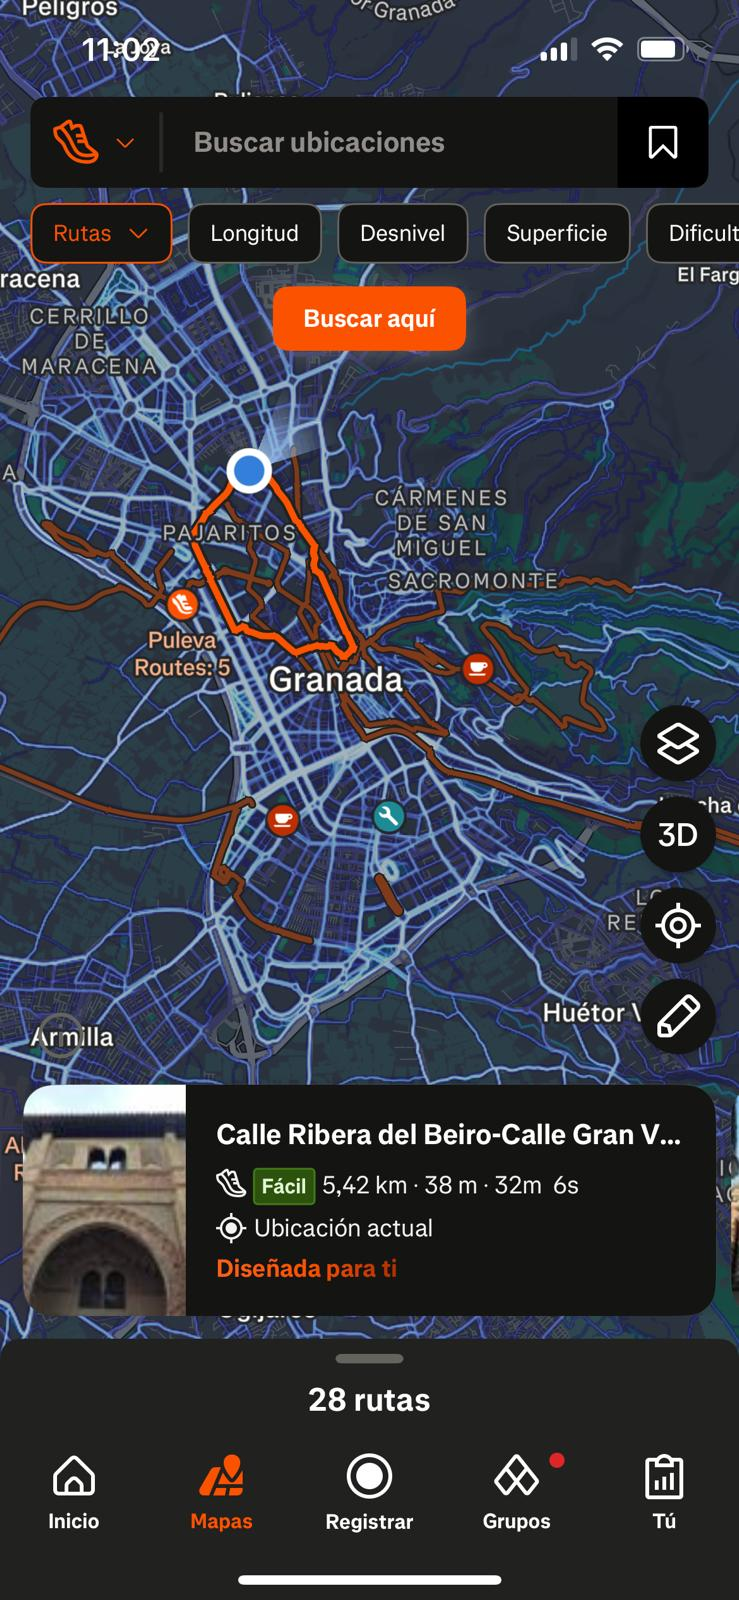
\includegraphics[width=0.5\textwidth]{fotos/strava.jpeg}
    \caption{Strava}
    \label{fig:Strava}
\end{figure} 
	\item \textbf{Whoop: €28}, de las aplicaciones esta es de lejos la más completa, permite medir, estrés, cansancio del usuario, calidad del entrenamiento, calidad de sueño, recuperación, edad de tu cuerpo según tus constantes, IA especializada para chatear y recibir consejos, etc. Sin embargo, es la que tiene la mensualidad más cara y solo funciona con un reloj de su marca, es decir, el usuario esta obligado a comprar ese reloj si quiere usar dicha app, el reloj en concreto vale 200€ mínimo.
\begin{figure}[H]
   \centering
    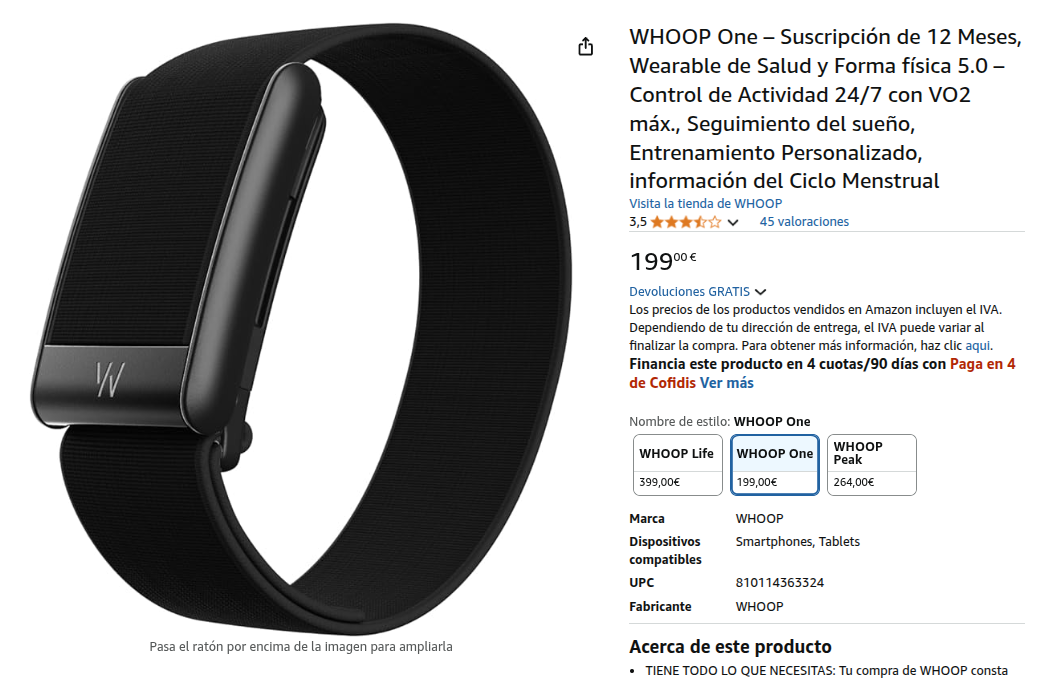
\includegraphics[width=0.5\textwidth]{fotos/Pulsera whoop.png}
    \caption{Pulsera whoop}
    \label{fig:Pulsera whoop}
\end{figure} 
\end{itemize}

Es verdad que algunas tienen versión gratuita, pero no ofrecen la totalidad de sus funcionalidades, de hecho, estas versiones suelen ser extremadamente limitadas. Otras aplicaciones como Garmin Connect, si que son gratuitas, pero te obligan a ceñirte a un smartwatch de la marca Garmin, los cuales su precio no baja de los 300€. 
La app presentada daría la mayoría de funcionalidades de pago de una manera gratuita y aporta su funcionalidad de medir de forma personalizada el rendimiento del deportista. También se añade una IA, una funcionalidad que no vista en muchas aplicaciones del sector y si existen, son de pago. La función de la inteligencia artificial sería la de aconsejar al usuario cuando este lo necesite, sobre su rendimiento y/o parámetros medidos durante su entrenamiento.
Para clarificar las diferencias con el resto de apps del mercado:

\begin{landscape}
\begin{figure}[H]
   \centering
    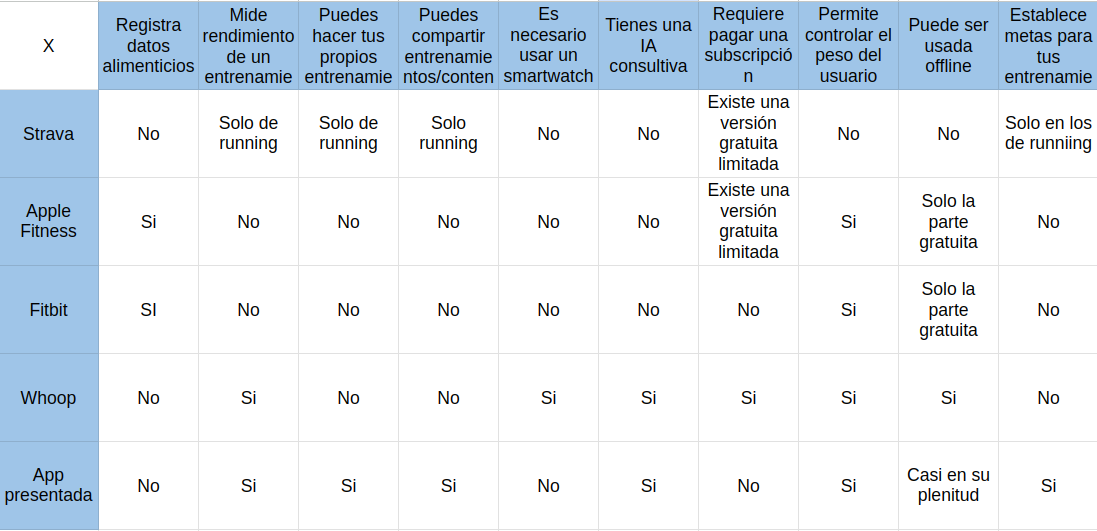
\includegraphics[width=1.65\textwidth]{tablas/tabla.png}
    \caption{Tabla comparativa}
    \label{fig:Tabla comparativa}
\end{figure} 
\end{landscape}

\section{Metodologías potenciales a aplicar}

Existen muchas formas de desarrollar software con sus respectivas ventajas, desventajas y forma de trabajar. En este caso, no voy a investigar sobre metodologías que usen la idea de prototipos(software que puede ser probado por el cliente durante el desarrollo):

\begin{itemize}
	\item \textbf{Cascada:} Es una forma de desarrollar de las más clásicas y lineales. Se hace una secuencia de fases de desarrollo, las cuales suelen ser diseño requisitos, diseño, implementación, pruebas, implementación y mantenimiento. Es una metodología fácil de entender y aplicar, eficaz para plazos de entrega estrictos. Sin embargo, no es flexible, si se encuentran fallos en la planificación o alguna de las fases, no hay mucho tiempo de reacción.
	\item \textbf{Desarrollo Ágil:} En lugar de una secuencia rígida de fases, se promuebe la flexibilidad, ya que se combina con reuniones con el cliente para obtener feedback del software funcional desarrollado entregado en dichas reuniones(no es un prototipo ya que solo es una demostración, no se le entrega para su uso durante el desarrollo), permitiendo corregir errores de planificación o en el propio software durante el desarrollo, sin perder mucho tiempo. Es necesario un buen feedback del cliente.
	\item \textbf{Lean Software Development: } Se basa en la idea de descartar todo aquello que no aporte valor para el cliente y quitarle importancia al desarrollo para ganar calidad y sostenibilidad en el tiempo al software. Esto se refleja en que primero se hace una investigación a fondo de todas las herramientas posibles a usar, su consecuente aprendizaje y en lo más tardio de todo esta la elección de que herramientos usar. Una vez hecha la elección, ya se puede empezar con el desarrollo.
	\item \textbf{V Model: } Es como el método cascada, pero antes de pasar a la siguiente fase se realizan las pruebas de la actual y no se procede hasta que estas estén válidas. Sigue teniendo las mismas desventajas que el modelo de cascada, pero es ideal para proyectos en los que es necesario una alta calidad.
	\item \textbf{Modelo en espiral: } En cada fase se realiza planificación, diseño, desarrollo y evaluación de riesgos. Es muy flexible y esta analizando constantemente los riesgos, pero se requiere cierta experiencia para su correcto empleo.
\end{itemize}

\section{Tecnologías potenciales para usar}

Para hablar de las tecnologías a emplear, lo voy a separar en las 3 partes importantes de la app la base de datos, backend y frontend.

\subsection{Base de datos}

En este punto vamos a hablar de las ventajas y desventajas entre usar BDs relacionales y no relacionales, así como las herramientas a emplear en cada una para desarrollar estos servicios.

\textbf{Relacionales:} Las bases de datos relacionales o SQL, como bien sabemos nos permiten guardar datos de una manera bien definida y ordenada, permitiendo asegurar la integridad de la información almacenada. Es muy buena opción, si se prefiere una escalabilidad vertical, es decir, aumentar la capacidad de procesamiento del servidor que va a albergar la BD. Algunas de los SGBDS existentes en la actualidad son:

\begin{itemize}
	\item MySQL
	\item Oracle Database
	\item SQL server(Microsoft)
	\item PostgreSQL
\end{itemize}

\textbf{No relacionales:} También llamadas NoSQL, sirven para trabajar con estructuras de datos semidefinidas o no definidas. Esto quiere decir que no siguen un esquema rígido, lo cuál puede complicar consultas complejas, pero permiten una gran escalabilidad horizontal, permiten añadir más servidores para que operen con la misma base de datos, por tanto aumentar el número de peticiones que puede atender. Cabe decir que dentro de este tipo de bases de datos existen varios subtipos, cada uno especializado en una cualidad:

\begin{itemize}
	\item Documentales(MongoDB): guardan los datos en un JSON
	\item Columnares(Cassandra): los datos no se guardan en filas, sino en columnas ,ideal para tratar grandes volumenes de datos por columnas
	\item Clave-Valor(DynamoDB): acceso rápido a los datos
	\item Graficas(Amazon Neptune): para tratar relaciones complejas
\end{itemize}

\subsection{Backend}

En el desarrollo del backend exiten varios frameworks que nos van a permitir un desarrollo rápido, eficaz y de calidad. Nuetro backend se va encargar principalmente de recibir y realizar peticiones de los clientes y/o consultas a la BD. Para ello se han investigado las siguientes herramientas:

\begin{itemize}
	\item Express.js(Node.js): muy escalable y alto rendimiento
	\item Django(Python): ideal para sistemas a gran escala
	\item Ruby on rails: el mejor en velociad de desarrollo
\end{itemize}

Existen más frameworks, pero he decidido investigar solo sobre aquellos que me permitan un desarrollo más ágil, el resto de herramientas como Spring Boot(Java) o Laravel(PHP), también son buenas herramientas, pero tengo más familiaridad con algunas de las herramientas anteriores.

\subsection{Frontend}

Como se dijo en la introducción, uno de los objetivos es que el software sea multiplataforma, así que se investigará sobre frameworks que me permitan esa capacidad:

\begin{itemize}
	\item Flutter(Dart): de las manos de Google, esta herramienta permite un desarrollo rápido ya que nos permite el hot reload y no tener que recompilar la app cada vez que haya un cambio. También es muy personalizable en lo que respecta a la UI.
	\item React Native(js): es un framework que extiende React, permitiendo hacer sentir aplicaciones en js como si fueran nativas.
	\item Xamarín(C\#): de Microsoft, esta herramienta es ideal para desarrolladores familiarizados con C\# y .NET, también es idóneo para el alto rendimiento y acceso a HW nativo.
\end{itemize}

\section{Trabajos relacionados}
El software libre y sus licencias \cite{gplv3} ha permitido llevar a cabo una expansión del aprendizaje de la informática sin precedentes.
